\documentclass[onlytextwidth]{beamer}
\usepackage[utf8]{inputenc}
\usepackage{microtype}
\usepackage{amsmath}
\usepackage{amssymb}
\usepackage[nomessages]{fp} %\FPeval{\var-name}{2*sin(pi/6)}
\usepackage{siunitx} %units in math. eg 20\milli\meter
\usepackage{yhmath} % for arcs, overparenth command
\usepackage{tikz} %graphics
\usetikzlibrary{quotes, angles}
%\usepackage{graphicx} already loaded by beamer class
%consider setting \graphicspath{{images/}}
%\parskip ?? to avoid paragraph indent
\usepackage{multicol} %may not need this package, just columns environment
\usepackage{venndiagram}

\subtitle[BECA]{Bronx Early College Academy}
\author[Huson]{Christopher J. Huson PhD}

\setbeamertemplate{headline}{\vskip2mm 
  BECA / \insertshortauthor \, / \inserttitle
  \hfill 
  \insertsection
  }

\title{Geometry Unit 1: Segments, Length, and Area}
\date{8-23 September 2022}

\begin{document}
\frame{\titlepage}

\section[Outline]{}
\frame{\tableofcontents}

\section{1.1 Segment addition \hfill 8 September}
\begin{frame}{Learning Target: I can measure my world}
  {CCSS: HSG.CO.A.1 Know precise geometric definitions \hfill \alert{1.1 Thursday 8 Sept}}
  \begin{block}{Do Now: Make simple measurements on paper}
    \begin{enumerate}
        \item Diagram the desks \emph{adjacent} to yours and their distances
        \item Early finishers: Calculate diagonal distances
        \item [ToDo:] add classroom desk image, diagram
    \end{enumerate}
    \end{block}
    Lesson: Points, line segments, length; Segment addition postulate \par 
    Routines and expectations \par \medskip
    Homework (on looseleaf, due tomorrow): 
    \begin{enumerate}
      \item Write for me your ``math autobiography.''
      \item Set one Math goal for the year.
      \item Optional: spicy absolute value worksheet
    \end{enumerate}
     \par \medskip
    
  \end{frame}

\begin{frame}{A \emph{diagram} is a simplied image representing a situation}
  {This is an example diagram of a desk arrangement}
  %\includegraphics[]{desk-layout-diagram}
  \begin{block}{When making diagrams}
    Include common elements: labels, titles, distances \par \medskip
  \end{block}
  \begin{description}
    \item[Conventions] Standard ways of doing things to make it easier to work with other people
    \item[Adjacent] Positioned next to each other
  \end{description} \vspace{2cm}
  Write down vocabulary and terminology in your notebook with definitions and examples. (I write new terms in \emph{italics})
  \end{frame}

\begin{frame}{\emph{Line segments} and their \emph{endpoints}}
  Points $P$, $A$, $B$, $C$, and line segments $\overline{AB}$, $\overline{BC}$ are shown. \vspace{1cm}
  \begin{columns}
    \column{0.7\textwidth}
      \begin{tikzpicture}
      \draw[fill] (5,2) circle [radius=0.05] node[below]{$P$};
      \draw[thick] (0,1)--(3,1);
      \draw[fill] (0,1) circle [radius=0.05] node[below]{$A$};
      \draw[fill] (3,1) circle [radius=0.05] node[below]{$B$};
      \draw[thick] (3,0)--(7,0);
      \draw[fill] (3,0) circle [radius=0.05] node[below]{$B$};
      \draw[fill] (7,0) circle [radius=0.05] node[below]{$C$};
    \end{tikzpicture}
    \column{0.3\textwidth}
      \emph{Given}:\par $AB=3$ \par $BC=4$
  \end{columns} \vspace{1cm}
  The \emph{length} of a line segment is the distance between the two endpoints. The length of segment $\overline{AB}$ is written $AB$ (no bar over).
  \end{frame}

\begin{frame}{A \emph{number line} is useful for calculating length or distance}
  {Take the difference in the points' values}
  Given $\overline{PQ}$ as shown on the number line.
    \begin{center}
      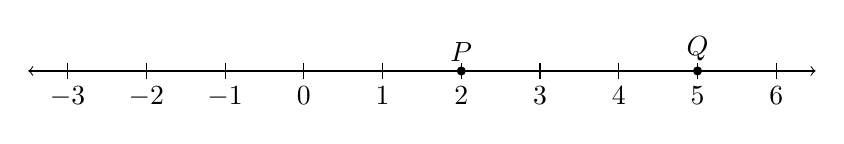
\begin{tikzpicture}
        \draw[<->] (-3.5,0)--(6.5,0);
        \foreach \x in {-3,...,6}
          \draw[shift={(\x,0)}] (0pt,-3pt)--(0pt,3pt) node[below=5pt]{$\x$};
        \draw[fill] (2,0) circle [radius=0.05] node[above]{$P$};
        \draw[fill] (5,0) circle [radius=0.05] node[above]{$Q$};
        \draw[thick] (2,0)--(5,0);
      \end{tikzpicture}
    \end{center}
    Find the distance on the number line between the points $P$ and $Q$. \par \bigskip
    \onslide<2> $$PQ = 5-2 =3$$ \par \bigskip
    Can a length be a negative number? \par \vspace{1cm}
    Most of the lengths on our problem sets are in centimeters.
  \end{frame}

\begin{frame}{Negative number practice on a number line}
  {Take the difference in the points' values. Check by counting the marks.}
  Given $\overline{MN}$ with $M(-1)$ and $N(3)$, as shown on the number line.
    \begin{center}
    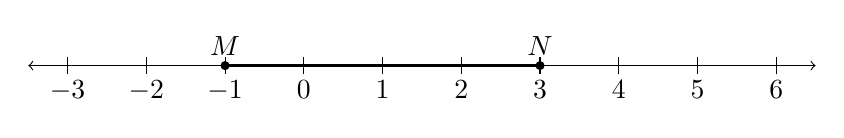
\begin{tikzpicture}
      \draw[<->] (-3.5,0)--(6.5,0);
      \foreach \x in {-3,...,6}
        \draw[shift={(\x,0)}] (0pt,-3pt)--(0pt,3pt) node[below=5pt]{$\x$};
      \draw[fill] (-1,0) circle [radius=0.05] node[above]{$M$};
      \draw[fill] (3,0) circle [radius=0.05] node[above]{$N$};
      \draw[thick] (-1,0)--(3,0);
    \end{tikzpicture}
    \end{center} \bigskip
    What is the length of the segment $\overline{MN}$? Show your work as an equation. \par \bigskip
    \onslide<2> $$MN=3- (-1)=4$$ \par \bigskip
    Why is ``minus a negative'' like adding a positive?
  \end{frame}

\begin{frame}{Decimal practice on a number line}
  {Mark the points then take the difference in the points' values.} \vspace{1cm}
  Given $\overline{GH}$ with $G(1)$ and $H(4.5)$.
    \begin{enumerate}
      \item Mark and label the points and segment on the number line.
      \item What is the length of the segment $\overline{GH}$? Show your work as an equation.
    \end{enumerate}
    \begin{center}
      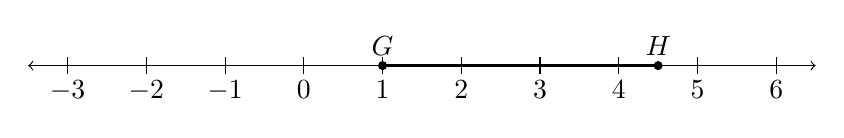
\begin{tikzpicture}
        \draw[<->] (-3.5,0)--(6.5,0);
        \foreach \x in {-3,...,6}
          \draw[shift={(\x,0)}] (0pt,-3pt)--(0pt,3pt) node[below=5pt]{$\x$};
        \onslide<2> 
          \draw[fill] (1,0) circle [radius=0.05] node[above]{$G$};
          \draw[fill] (4.5,0) circle [radius=0.05] node[above]{$H$};
          \draw[thick] (1,0)--(4.5,0);
      \end{tikzpicture}
    \end{center} \bigskip
    \onslide<2> {$$GH= 4.5 - 1 = 3.5$$} \vspace{2cm}
  \end{frame}

\begin{frame}{Take class notes in a composition book}
  {Copy definitions using your own words. Write down example diagrams and problems}
  Terminology:
    \begin{description}
      \item[Point] A location, has no size; label with capital letter, $P$
      \item[Endpoint] A point at the end of a line segment
      \item[Line segment] Two points and all the points between them; label with \emph{endpoints} and a bar, e.g. $\overline{AB}$
      \item[Distance] The positive difference between two points on a number line (length is the same thing). $AB=3$ inches
      \item[Number line] A line with lengths marked on it
      \item[Conventions] Standard ways of doing things to make it easier to work with other people
      \item[Diagram] Simplified image of a situation
      \item[Adjacent] Positioned next to each other
    \end{description}
  \end{frame}

\begin{frame}{Spicy: \emph{Absolute value} is the distance from a point to zero}
  {``Spicy'', or extension topics, must be written in your notebook, but homework and tests are optional.}
    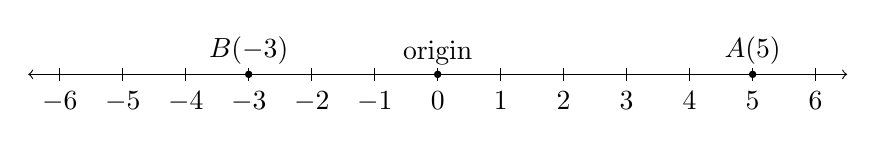
\begin{tikzpicture}[scale=0.8]
      \draw[<->] (-6.5,0)--(6.5,0);
      \foreach \x in {-6,...,6}
        \draw[shift={(\x,0)}] (0pt,-3pt)--(0pt,3pt) node[below=5pt]{$\x$};
      \draw[fill] (0,0) circle [radius=0.05] node[above]{origin};
      \draw[fill] (5,0) circle [radius=0.05] node[above]{$A(5)$};
      \draw[fill] (-3,0) circle [radius=0.05] node[above]{$B(-3)$};
    \end{tikzpicture} \par \bigskip
    The absolute value of 5 is 5. $|5|=5$ \par \bigskip
    The absolute value of $-3$ is 3. $|-3|=3$ \par \bigskip
    The absolute value of a number is always a positive number, or zero  \par \smallskip
    Write the absolute value of a number $x$ using vertical bars $|x|$ or $abs(x)$
  \end{frame}

\section{1.2 Solve for length \hfill 9 September}
\begin{frame}{Learning Target: I can solve for segment lengths}
  {CCSS: HSG.CO.A.1 Know precise geometric definitions  \hfill \alert{1.2 Friday 9 September}}
  Do Now: Given $A(1)$, $B(4)$, $C(6)$. \par \medskip
  Write down $AB$, $BC$, and $AC$.
  \begin{center}
    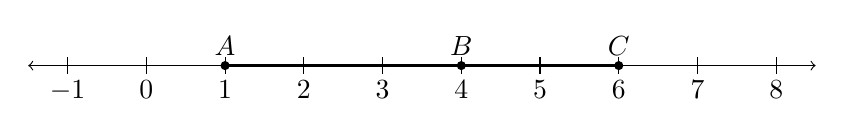
\begin{tikzpicture}
      \draw[<->] (-1.5,0)--(8.5,0);
      \foreach \x in {-1,...,8}
        \draw[shift={(\x,0)}] (0pt,-3pt)--(0pt,3pt) node[below=5pt]{$\x$};
      \draw[fill] (1,0) circle [radius=0.05] node[above]{$A$};
      \draw[fill] (4,0) circle [radius=0.05] node[above]{$B$};
      \draw[fill] (6,0) circle [radius=0.05] node[above]{$C$};
      \draw[thick] (1,0)--(6,0);
    \end{tikzpicture}
  \end{center} \vspace{1cm}
  Lesson: Segment addition, solving algebraic models \par \medskip
  Homework: Problem set 1.2 (plus optional spicy worksheet)
  \end{frame}

\begin{frame}{Lengths add up on a straight line}
  {\emph{Segment Addition Postulate}}
  Shown \emph{collinear} points $A$, $B$, $C$. Given $AB=3$, $BC=4$. \par \medskip
  Find $AC$.
    \begin{center}
      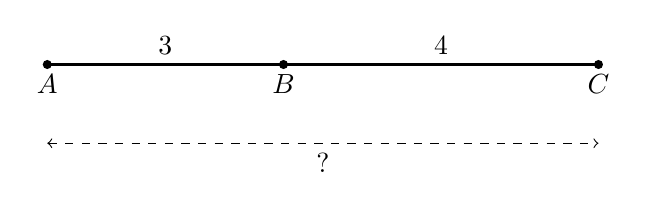
\begin{tikzpicture}
        \draw[fill] (0,0) circle [radius=0.05] node[below]{$A$};
        \draw[thick] (0,0)--(7,0);
        \draw[fill] (3,0) circle [radius=0.05] node[below]{$B$};
        \draw[fill] (7,0) circle [radius=0.05] node[below]{$C$};
        \node at (1.5,0) [above]{$3$};
        \node at (5,0) [above]{$4$};
        \draw[<->, dashed] (0,-1)--(7,-1);
        \node at (3.5,-1) [below]{$?$};
      \end{tikzpicture}
    \end{center} \vspace{1cm}
    Definitions:
    \begin{description}
      \item[Collinear] Points that lie on the same straight line
      \item[Postulate] A rule that we assume is true
    \end{description}
  \end{frame}

\begin{frame}{Use a variable ($x$) to represent an unknown value}
  {An equation is a \emph{model} of a situation}
  Given collinear points $Q$, $R$, $S$, with $QR=11$, $QS=20$. \par \medskip
  Find $RS$.
  \begin{center}
    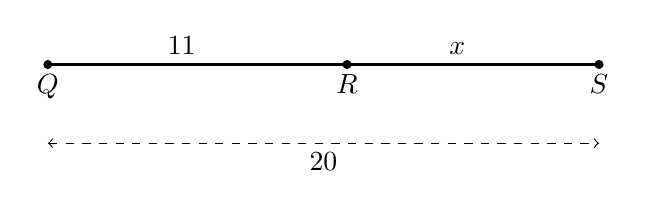
\begin{tikzpicture}
      \draw[fill] (0,0) circle [radius=0.05] node[below]{$Q$};
      \draw[thick] (0,0)--(7,0);
      \draw[fill] (3.8,0) circle [radius=0.05] node[below]{$R$};
      \draw[fill] (7,0) circle [radius=0.05] node[below]{$S$};
      \node at (1.7,0) [above]{$11$};
      \node at (5.2,0) [above]{$x$};
      \draw[<->, dashed] (0,-1)--(7,-1);
      \node at (3.5,-1) [below]{$20$};
    \end{tikzpicture}
  \end{center}
  \begin{enumerate}
    \item How would you check your answer?
    \item Which equation represents the situation? \medskip
    \begin{columns}
      \column{0.5\textwidth}
      \hspace{2cm} $11 + x = 20$
      \column{0.5\textwidth}
      $x = 20 - 11$
    \end{columns}
  \end{enumerate}
  \end{frame}

\begin{frame}{Step-by-step modeling}
  Given $\overline{JKL}$, $JK=2x+3$, $KL=5$, $JL=12$. Find ${x}$.
  \begin{center}
  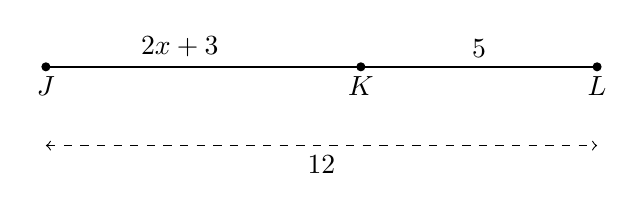
\begin{tikzpicture}
    \draw[thick] (0,0)--(7,0);
    \draw[fill] (0,0) circle [radius=0.05] node[below]{$J$};
    \draw[fill] (4,0) circle [radius=0.05] node[below]{$K$};
    \draw[fill] (7,0) circle [radius=0.05] node[below]{$L$};
    \node at (1.7,0) [above]{$2x+3$};
    \node at (5.5,0) [above]{$5$};
    \draw[<->, dashed] (0,-1)--(7,-1);
    \node at (3.5,-1) [below]{$12$};
  \end{tikzpicture}
  \end{center}
  \begin{enumerate}
    \item Write down an equation to represent the situation. \vspace{0.5cm}
    \item Solve for $x$. \vspace{0.5cm}
    \item Check your answer.
  \end{enumerate} \vspace{1cm}
  \end{frame}

\begin{frame}{The diagram may be given, or you may have to sketch it}
  {Write the steps in your notebook}
  Given $\overline{JKL}$, $JK=2x+3$, $KL=5$, $JL=12$. Find ${x}$.
  \begin{center}
    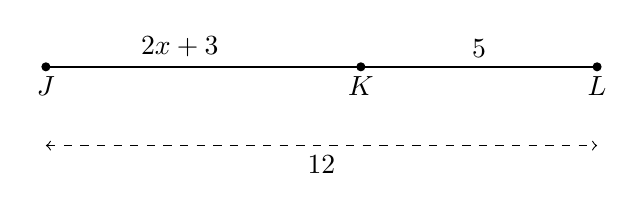
\begin{tikzpicture}
      \draw[thick] (0,0)--(7,0);
      \draw[fill] (0,0) circle [radius=0.05] node[below]{$J$};
      \draw[fill] (4,0) circle [radius=0.05] node[below]{$K$};
      \draw[fill] (7,0) circle [radius=0.05] node[below]{$L$};
      \node at (1.7,0) [above]{$2x+3$};
      \node at (5.5,0) [above]{$5$};
      \draw[<->, dashed] (0,-1)--(7,-1);
      \node at (3.5,-1) [below]{$12$};
    \end{tikzpicture}
  \end{center}
  \begin{columns}
    \column{0.4\textwidth}
      \[JK+KL=JL\]
      \[(2x+3)+5=12\]
      \[2x+8=12\]
      \[2x=4\]
      \[x=2\]
      \[2(2)+3+5=12?\]
    \column{0.6\textwidth}
      \begin{enumerate}
        \item Sketch and label the situation
        \item Write a geometric equation
        \item Substitute algebraic values
        \item Solve for $x$
        \item Answer the question
        \item \alert{Check} your answer
      \end{enumerate}
    \end{columns}
  \end{frame}

\begin{frame}{Mark the diagram, find $x$, answer $AB=?$}
  Given $\overline{ABC}$, $AB=3x-7$, $BC=x+5$, $AC=14$. \vspace{1cm}
  \begin{center}
      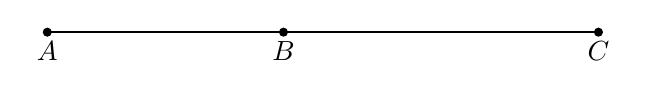
\begin{tikzpicture}
      \draw[thick] (0,0)--(7,0);
      \draw[fill] (0,0) circle [radius=0.05] node[below]{$A$};
      \draw[fill] (3,0) circle [radius=0.05] node[below]{$B$};
      \draw[fill] (7,0) circle [radius=0.05] node[below]{$C$};
    \end{tikzpicture}
  \end{center} 
  Find ${AB}$.\vspace{3cm}
  \end{frame}

\begin{frame}{More practice: Solve an equation with $x$ on both sides}
  Given $\overrightarrow{DEF}$, $DE=x+1$, $EF=9$, $DF=3x$. Find ${DE}$. \vspace{1cm}
  \begin{center}   
  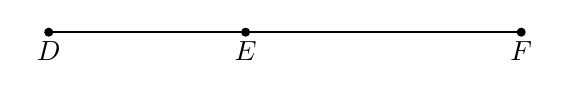
\begin{tikzpicture}
      \draw[thick] (0,0)--(6,0);
      \draw[fill] (0,0) circle [radius=0.05] node[below]{$D$};
      \draw[fill] (2.5,0) circle [radius=0.05] node[below]{$E$};
      \draw[fill] (6,0) circle [radius=0.05] node[below]{$F$};
    \end{tikzpicture}
  \end{center} \vspace{3cm}
  \end{frame}

\begin{frame}{Lengths in a straight line add up}
  {Check your notebook for completeness}
  \begin{block}{Segment Addition Postulate}
    Mathematics is constructed of fundamental rules or postulates, and basic objects like points, lines, and numbers.
  \end{block} \vspace{1cm}
    Vocabulary:
    \begin{description}
      \item[Collinear] Points that lie on the same straight line
      \item[Postulate] A rule that we assume is true (also called \emph{axioms})
      \item[Modeling] Using an equation (algebra) to represent a situation in a simplified way
      \item[Check] Substitute the value of $x$ into the equation to test whether it is correct
    \end{description}
  \end{frame}

\begin{frame}{Spicy: Fractional \emph{coefficients}}
  Given $\overline{ABC}$, $AB=\frac{1}{2}x$, $BC=x$, $AC=21$. Find ${x}$.\vspace{1cm}
  \begin{center}   
  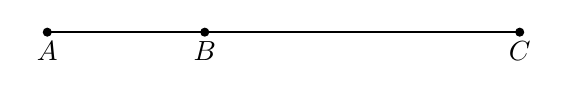
\begin{tikzpicture}
      \draw[thick] (0,0)--(6,0);
      \draw[fill] (0,0) circle [radius=0.05] node[below]{$A$};
      \draw[fill] (2,0) circle [radius=0.05] node[below]{$B$};
      \draw[fill] (6,0) circle [radius=0.05] node[below]{$C$};
    \end{tikzpicture}
  \end{center} \vspace{3cm}
  \begin{description}
    \item[Term] An expression representing a number, for example $\frac{1}{2}x$
    \item[Variable] The unknown value represented by a letter ($x$)
    \item[Coefficient] The fixed number in front of the variable. (e.g. $\frac{1}{2}$) 
    \end{description}
  \end{frame}

\section{1.3 Terminology and notation \hfill 12 September}
\begin{frame}{Learning Target: I can use geometric conventions}
  {CCSS: HSG.CO.A.1 Know precise geometric definitions \hfill \alert{1.3 Monday 12 Sept}}
  Do Now: Given collinear points $A$, $B$, $C$, with $AB=7$, $AC=13$.
  \begin{center}
    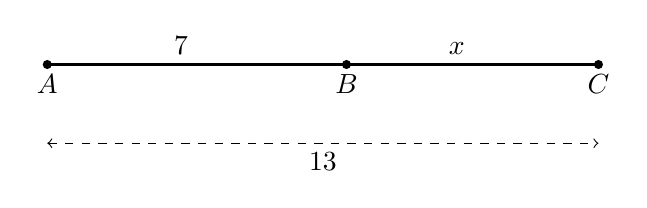
\begin{tikzpicture}
      \draw[fill] (0,0) circle [radius=0.05] node[below]{$A$};
      \draw[thick] (0,0)--(7,0);
      \draw[fill] (3.8,0) circle [radius=0.05] node[below]{$B$};
      \draw[fill] (7,0) circle [radius=0.05] node[below]{$C$};
      \node at (1.7,0) [above]{$7$};
      \node at (5.2,0) [above]{$x$};
      \draw[<->, dashed] (0,-1)--(7,-1);
      \node at (3.5,-1) [below]{$13$};
    \end{tikzpicture}
  \end{center}
  \begin{enumerate}
    \item Circle the equation that most simply represents the situation. \medskip
    \begin{columns}[c]
      \column{0.6\textwidth}
      \qquad \hspace{2cm} $7 + x = 13$
      \column{0.4\textwidth}
      $x = 13 - 7$
    \end{columns}
    \item Find $BC$.
  \end{enumerate} \vspace{2cm}
  Lesson: Vocabulary and notation
  \end{frame}

\begin{frame}{Write down an example of each geometric object.}
{Use proper notation.}
  \begin{enumerate}
    \item point
    \item line segment
    \item endpoint
    \item three collinear points
      \begin{tikzpicture}
      \draw[thick] (0,2)--(3,1);
      \draw[fill] (0,2) circle [radius=0.05] node[below]{$R$};
      \draw[fill] (3,1) circle [radius=0.05] node[below]{$S$};
      \draw[thick] (5,0)--(8,3);
      \draw[fill] (5,0) circle [radius=0.05] node[above left]{$T$};
      \draw[fill] (7,2) circle [radius=0.05] node[above left]{$U$};
      \draw[fill] (8,3) circle [radius=0.05] node[above left]{$V$};
    \end{tikzpicture}
    \item Given $TU=1.4$, $UV=0.6$. Find $TV$. (label the diagram first)
  \end{enumerate}
  \end{frame}

\begin{frame}{More definitions: lines, rays, planes}
  A \emph{line} extends infinitely in both directions, $\overleftrightarrow{AB}$. \par
  (sometimes labeled with a small letter, for example, line $k$)
  \begin{center}
    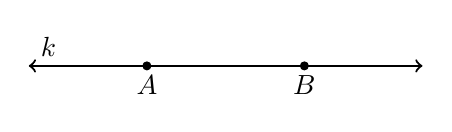
\begin{tikzpicture}
      \draw[<->, thick] (0,1)--(5,1);
      \node at (0.25, 1)[above]{$k$};
      \draw[fill] (1.5,1) circle [radius=0.05] node[below]{$A$};
      \draw[fill] (3.5,1) circle [radius=0.05] node[below]{$B$};
    \end{tikzpicture}
  \end{center}
  A \emph{ray} has one endpoint and extends infinitely in one direction, $\overrightarrow{CD}$.
    \begin{center}
    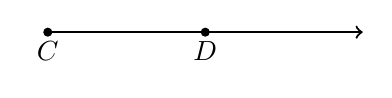
\begin{tikzpicture}
      \draw[->, thick] (3,0)--(7,0);
      \draw[fill] (3,0) circle [radius=0.05] node[below]{$C$};
      \draw[fill] (5,0) circle [radius=0.05] node[below]{$D$};
      \end{tikzpicture}
    \end{center}
  A \emph{plane} is flat and extends infinitely in two directions, $p$.
  \begin{center}
    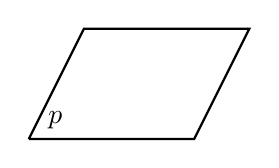
\begin{tikzpicture}[scale=0.7]
      \draw[thick](0,0) node[above right]{$\ p$} --(3,0)--(4,2)--(1,2)--(0,0);
    \end{tikzpicture}
    \end{center}
  \end{frame}

\begin{frame}{\emph{Opposite rays} are collinear rays with a common endpoint.}
  \begin{columns}
    \column{0.4\textwidth} 
      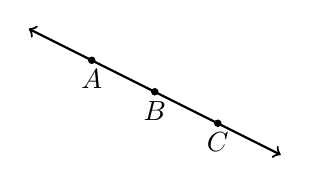
\begin{tikzpicture}[scale=.8]
        \draw[<->, thick] (0,2)--(4,0);
        \draw[fill] (1,1.5) circle [radius=0.05] node[below]{$A$};
        \draw[fill] (2,1) circle [radius=0.05] node[below]{$B$};
        \draw[fill] (3,0.5) circle [radius=0.05] node[below]{$C$};
      \end{tikzpicture}
    \column{0.6\textwidth} 
      $\overrightarrow{BA}$ and $\overrightarrow{BC}$ are opposite rays.
  \end{columns}
  \begin{columns}
    \column{0.4\textwidth}
      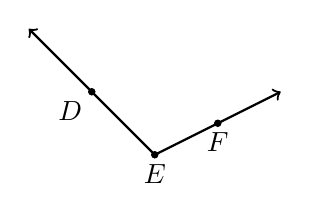
\begin{tikzpicture}[scale=.8]
        \draw[<->, thick] (0,2)--(2,0)--(4,1);
        \draw[fill] (1,1) circle [radius=0.05] node[below left]{$D$};
        \draw[fill] (2,0) circle [radius=0.05] node[below]{$E$};
        \draw[fill] (3,0.5) circle [radius=0.05] node[below]{$F$};
      \end{tikzpicture}
    \column{0.6\textwidth}
      These rays do not make a straight line.
  \end{columns} \bigskip
  \begin{columns}
    \column{0.4\textwidth}
      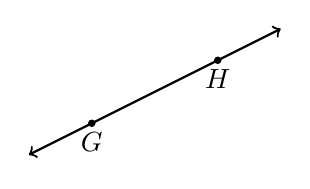
\begin{tikzpicture}[scale=.8]
        \draw[<->, thick] (0,-2)--(4,0);
        \draw[fill] (1,-1.5) circle [radius=0.05] node[below]{$G$};
        \draw[fill] (3,-0.5) circle [radius=0.05] node[below]{$H$};
      \end{tikzpicture}
    \column{0.6\textwidth}
      The rays $\overrightarrow{GH}$ and $\overrightarrow{HG}$ do not share a common endpoint.
  \end{columns}
  \end{frame}

\begin{frame}{Several objects are shown in a plane}{Circle true or false}
  \begin{enumerate}
    \item T \quad F \quad The name of the plane is $m$.
    \item T \quad F \quad The line $\overleftrightarrow{WY}$ is in the plane.
    \item T \quad F \quad The ray $\overrightarrow{WX}$ is shown in the plane.
    \item T \quad F \quad Points $W$, $X$, and $Z$ are collinear.
    \item T \quad F \quad $\overleftrightarrow{WY}$ and $\overleftrightarrow{YW}$ are the same line.
    \end{enumerate}
    \begin{center}
      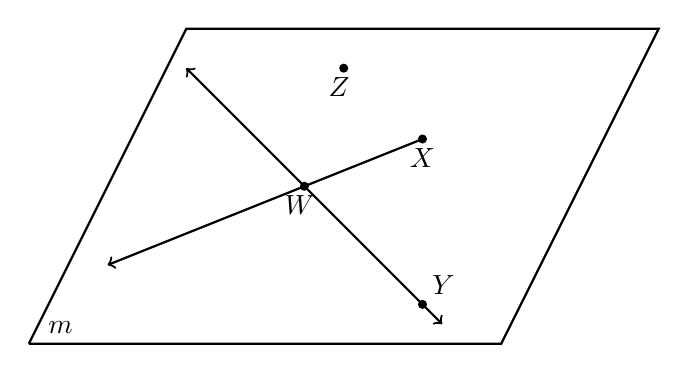
\begin{tikzpicture}
      \draw[thick](0,0) node[above right]{$\ m$} --(6,0)--(8,4)--(2,4)--(0,0);
      \draw[<-, thick] (1,1)--(5,2.6);
      \draw[fill] (4, 3.5) circle [radius=0.05] node[below]{$Z \ $};
      \draw[fill] (3.5,2) circle [radius=0.05] node[below]{$W \ $};
      \draw[fill] (5,2.6) circle [radius=0.05] node[below]{$X$};
      \draw[<->, thick] (2,3.5)--(5.25,.25);
      \draw[fill] (5,0.5) circle [radius=0.05] node[above right]{$Y \ $};
    \end{tikzpicture}
  \end{center}
  \end{frame}

\begin{frame}{More definitions: intersections, coplanar}
  Two lines \emph{intersect} if they cross. Their common point is the \emph{intersection}. 
  (shown here, lines $j$ and $k$ intersect at point $P$)
    \begin{center}
      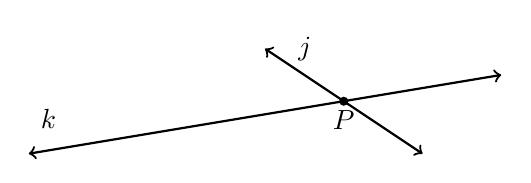
\begin{tikzpicture}
          \draw[<->, thick] (0,0)--(6,1);
          \draw[<->, thick] (3,1.333)--(5,0);
          \node at (0.25, 0.2)[above]{$k$};
          \node at (3.3, 1.333)[right]{$j$};
          \draw[fill] (4,0.666) circle [radius=0.05] node[below]{$P$};
        \end{tikzpicture}
      \end{center}
      \emph{Coplanar} means to lie in the same plane. Three points are always coplanar, but four points may not be.
      \begin{center}
        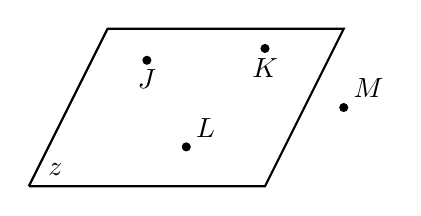
\begin{tikzpicture}[scale=1]
        \draw[thick](0,0) node[above right]{$\ z$} --(3,0)--(4,2)--(1,2)--(0,0);
        \draw[fill] (3,1.75) circle [radius=0.05] node[below]{$K$};
        \draw[fill] (1.5,1.6) circle [radius=0.05] node[below]{$J$};
        \draw[fill] (2,0.5) circle [radius=0.05] node[above right]{$L$};
        \draw[fill] (4,1) circle [radius=0.05] node[above right]{$M$};
      \end{tikzpicture}
    \end{center}
  \end{frame}

\begin{frame}{Learn and practice using formal language and notation}
  \begin{description}%[itemsep=1cm]
    \item[Line] An infinite collection of points extending straight in both directions indefinitely, $\overleftrightarrow{AB}$ or $l$
    \item[Ray] An endpoint and half of a straight line extending away from the endpoint, $\overrightarrow{JK}$
    \item[Plane] A flat surface extending infinitely in two dimensions, $p$
    \item[Opposite rays] Collinear rays with a common endpoint. 
    \item[Coplanar] Points or objects all in the same plane
    \item[Intersection] Where two lines cross, the common point
  \end{description}
  \end{frame}

\begin{frame}{Spicy: Which is the more efficient method, \\ \qquad \emph{distribute} or multiply both sides by 3?}
  \begin{columns}[c]
    \column{0.6\textwidth} $\frac{2}{3}(x+5)=4$
    \column{0.4\textwidth} $\frac{2}{3}(x+5)=4$
  \end{columns} \vspace{3cm}
  \begin{description}
    \item[Distribute] Multiply both terms in parentheses by the coefficient
    \item[Numerator] The top of a fraction (i.e. $p$ in $\frac{p}{q}$)
    \item[Denominator] The bottom of a fraction (i.e. $q$ in $\frac{p}{q}$)
    \item[LCD] Converting to the \emph{Lowest Common Denominator} is the most efficient way to add fractions
  \end{description}
  \end{frame}

\section{1.4 Midpoint and bisector \hfill 13 September}
\begin{frame}{Learning Target: I can \emph{bisect} a length}
  {CCSS: HSG.CO.A.1 Know precise geometric definitions  \hfill \alert{1.4 Tuesday 13 Sept}}
  \begin{block}{Do Now: Circle or mark each object in the plane}
    \begin{enumerate} 
      \item The point $H$
      \item The ray $\overrightarrow{JL}$
      \item The name of the plane shown
      \end{enumerate}
    \begin{center}
    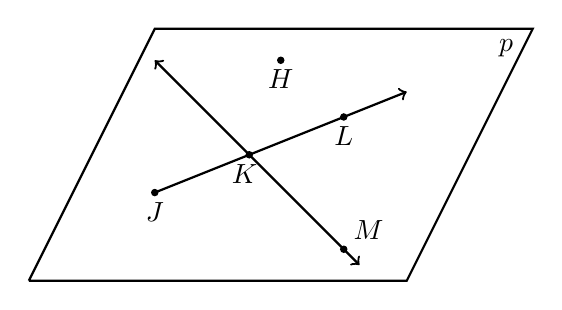
\begin{tikzpicture}[scale=0.8]
      \draw[thick](0,0)--(6,0)--(8,4) node[below left]{$p \ $} --(2,4)--(0,0);
      \draw[->, thick] (2, 1.4)--(6,3);
      \draw[fill] (4, 3.5) circle [radius=0.05] node[below]{$H$};
      \draw[fill] (2, 1.4) circle [radius=0.05] node[below]{$J$};
      \draw[fill] (3.5,2) circle [radius=0.05] node[below]{$K \ $};
      \draw[fill] (5,2.6) circle [radius=0.05] node[below]{$L$};
      \draw[<->, thick] (2,3.5)--(5.25,.25);
      \draw[fill] (5,0.5) circle [radius=0.05] node[above right]{$M \ $};
    \end{tikzpicture}
    \end{center}
    \end{block}
    Lesson: Midpoint, congruence, bisection
  \end{frame}

\begin{frame}{The point $B$ \emph{bisects} the segment $\overline{AC}$}
  \begin{block}{Point $B$ is in the exact middle between $A$ and $C$}
    Given $AB=x+2$, $BC=11$. Find $x$.
    \begin{center}
    \begin{tikzpicture}
      \draw[fill] (0,0) circle [radius=0.05] node[below]{$A$};
      \draw[thick] (0,0)--(7,0);
      \draw[fill] (3.5,0) circle [radius=0.05] node[below]{$B$};
      \draw[fill] (7,0) circle [radius=0.05] node[below]{$C$};
      \node at (1.7,0.5) [above]{$x+2$};
      \node at (5.2,0.5) [above]{$11$};
    \end{tikzpicture}
    \end{center}
    \end{block}
    Hint: The line segment is split into two equal lengths. \vspace{3cm}
  \end{frame}

\begin{frame}{The \emph{midpoint} of a line segment}
  Given $\overline{ABC}$, with $AB=2x+2$, $AC=20$. $AB=BC$ \\[0.15in]
  Find $x$.
  \begin{center}
    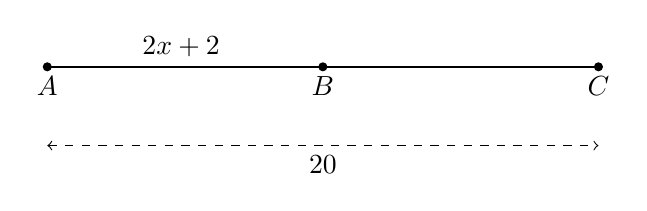
\begin{tikzpicture}
      \draw[fill] (0,0) circle [radius=0.05] node[below]{$A$};
      \draw[thick] (0,0)--(7,0);
      \draw[fill] (3.5,0) circle [radius=0.05] node[below]{$B$};
      \draw[fill] (7,0) circle [radius=0.05] node[below]{$C$};
      \node at (1.7,0) [above]{$2x+2$};
      \draw[<->, dashed] (0,-1)--(7,-1);
      \node at (3.5,-1) [below]{$20$};
    \end{tikzpicture}
    \end{center} \vspace{2cm}
  \end{frame}

\begin{frame}{A \emph{bisector} creates two line segments with the same length}
  {\emph{Congruent} line segments are the same length}
  Given point $B$ is the midpoint of $\overline{AC}$, with $AB=x+7$, $BC=17$.
  Find $x$.
    \begin{center}
      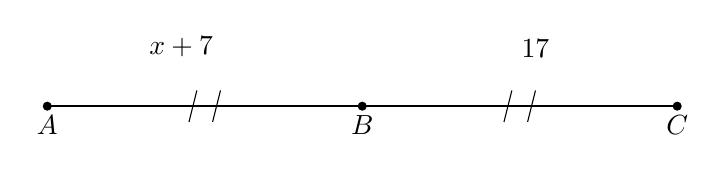
\begin{tikzpicture}
        \draw[thick] (0,0)--(8,0);
        \draw[fill] (0,0) circle [radius=0.05] node[below]{$A$};
        \draw[fill] (4,0) circle [radius=0.05] node[below]{$B$};
        \draw[fill] (8,0) circle [radius=0.05] node[below]{$C$};
        \node at (1.7,0.5) [above]{$x+7$};
        \node at (6.2,0.5) [above]{$17$};
        \draw (1.8,-0.2)--(1.9,0.2);
        \draw (2.1,-0.2)--(2.2,0.2);
        \draw (5.8,-0.2)--(5.9,0.2);
        \draw (6.1,-0.2)--(6.2,0.2);
      \end{tikzpicture}
    \end{center} \vspace{2cm}
  The \emph{midpoint} or \emph{bisector} of a line segment divides it exactly in half. \par \medskip
  \emph{Congruent} means equal in length, $\overline{AB} \cong \overline{BC}$ (also $AB=BC$)\par
  Mark congruent segments in diagrams with cross ``\emph{hash}" marks.
  \end{frame}

\begin{frame}{Check your notes}{$M$ bisects $\overline{PQ}$}
  \begin{center}
    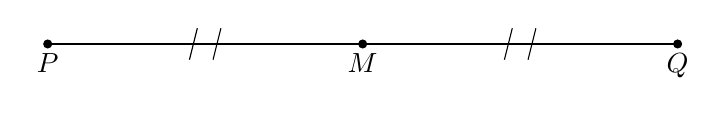
\begin{tikzpicture}
      \draw[thick] (0,0)--(8,0);
      \draw[fill] (0,0) circle [radius=0.05] node[below]{$P$};
      \draw[fill] (4,0) circle [radius=0.05] node[below]{$M$};
      \draw[fill] (8,0) circle [radius=0.05] node[below]{$Q$};
      \draw (1.8,-0.2)--(1.9,0.2);
      \draw (2.1,-0.2)--(2.2,0.2);
      \draw (5.8,-0.2)--(5.9,0.2);
      \draw (6.1,-0.2)--(6.2,0.2);
    \end{tikzpicture}
  \end{center} \vspace{1cm}
  \begin{description}
    \item[Bisect] Divide exactly in half
    \item[Midpoint] The point in the exact middle of a line segment
    \item[Congruent] Equal in length or measure. $\overline{AB} \cong \overline{BC}$
    \item[Hash marks] Mark congruent segments with small crossways lines (also called ``tick'' marks)
  \end{description}
  \end{frame}

\begin{frame}{Spicy: \emph{Trisect} a segment into three congruent parts}
  Points $B$ and $C$ trisect segment $\overline{AD}$ with segment lengths as shown. \par \medskip 
  Find $x$.
  \begin{center}
    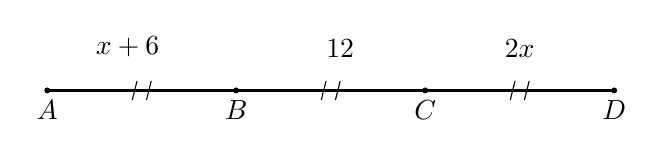
\begin{tikzpicture}[scale=0.6]
      \draw[thick] (0,0)--(12,0);
      \draw[fill] (0,0) circle [radius=0.05] node[below]{$A$};
      \draw[fill] (4,0) circle [radius=0.05] node[below]{$B$};
      \draw[fill] (8,0) circle [radius=0.05] node[below]{$C$};
      \draw[fill] (12,0) circle [radius=0.05] node[below]{$D$};
      \node at (1.7,0.5) [above]{$x+6$};
      \node at (6.2,0.5) [above]{$12$};
      \node at (10,0.5) [above]{$2x$};
      \draw (1.8,-0.2)--(1.9,0.2);
      \draw (2.1,-0.2)--(2.2,0.2);
      \draw (5.8,-0.2)--(5.9,0.2);
      \draw (6.1,-0.2)--(6.2,0.2);
      \draw (9.8,-0.2)--(9.9,0.2);
      \draw (10.1,-0.2)--(10.2,0.2);
    \end{tikzpicture}
  \end{center} \vspace{2cm}
  \begin{description}
    \item[Trisect] Divide exactly in three equal parts
    \item[Partition] Cut into parts (not necessarily evenly)
  \end{description}
  \end{frame}

\section{1.5 Equilateral and isosceles triangles, perimeter \hfill 15 September}
\begin{frame}{Learning Target: I can work with objects having congruent parts}
  {CCSS: HSG.CO.A.1 Know precise geometric definitions  \hfill \alert{1.5 Thursday 15 Sept}}
    \begin{block}{Do Now: Given $\overline{ST}$ with $S(-2)$ and $T(4)$}
      \begin{center}
      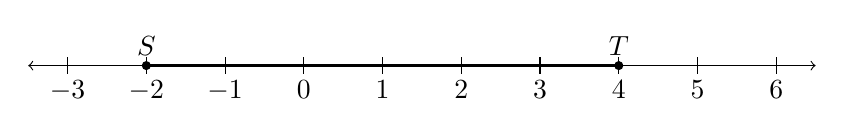
\begin{tikzpicture}
        \draw[<->] (-3.5,0)--(6.5,0);
        \foreach \x in {-3,...,6}
          \draw[shift={(\x,0)}] (0pt,-3pt)--(0pt,3pt) node[below=5pt]{$\x$};
        \draw[fill] (-2,0) circle [radius=0.05] node[above]{$S$};
        \draw[fill] (4,0) circle [radius=0.05] node[above]{$T$};
        \draw[thick] (-2,0)--(4,0);
      \end{tikzpicture}
      \end{center}
    What is the length of the segment $\overline{ST}$? Show your work as an equation.
    \end{block} \vspace{2cm}
    Lesson: Perimeter, congruent line segments in rectangles \& isosceles triangles
  \end{frame}

\begin{frame}{Negative number practice on a number line}
  {Take the difference in the points' values. Check by counting the marks.}
  Given $\overline{ST}$ with $S(-2)$ and $T(4)$, as shown on the number line.
  \begin{center}
    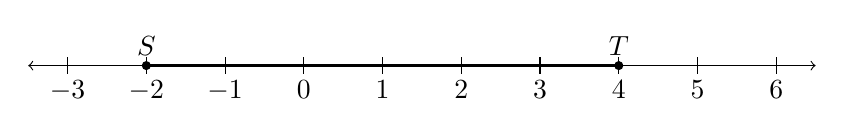
\begin{tikzpicture}
      \draw[<->] (-3.5,0)--(6.5,0);
      \foreach \x in {-3,...,6}
        \draw[shift={(\x,0)}] (0pt,-3pt)--(0pt,3pt) node[below=5pt]{$\x$};
      \draw[fill] (-2,0) circle [radius=0.05] node[above]{$S$};
      \draw[fill] (4,0) circle [radius=0.05] node[above]{$T$};
      \draw[thick] (-2,0)--(4,0);
    \end{tikzpicture}
  \end{center}
  What is the length of the segment $\overline{ST}$? Show your work as an equation. \par \bigskip
  \qquad Solution 
  $$ST=4-(-2)=6$$
  \par \vspace{2cm}
  Why is ``minus a negative" the same as add a positive? 
  \end{frame}

\begin{frame}{An \emph{isosceles} triangle has two congruent sides}
  Given isosceles $\triangle ABC$. Which two sides are congruent? \par \medskip
  Write your answer using symbols (i.e. two segments and $\cong$) \par
  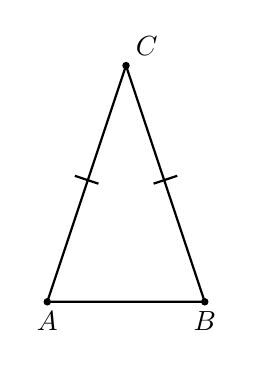
\begin{tikzpicture}[scale=0.5]
    \draw[thick](0,0)--(4,0)--(2,6)--cycle;
    \draw[fill] (0,0) circle [radius=0.08] node[below]{$A$};
    \draw[fill] (4,0) circle [radius=0.08] node[below]{$B$};
    \draw[fill] (2,6) circle [radius=0.08] node[above right]{$C$};
    \draw[thick] (0.7,3.2)--(1.3,3); %tick mark
    \draw[thick] (2.7,3)--(3.3,3.2); %tick mark
  \end{tikzpicture}
  \end{frame}

\begin{frame}{On the diagram mark the congruent line segments with tick marks.}
  Given isosceles $\triangle STU$ with $\overline{ST} \cong \overline{TU}$. 
  \begin{center}
  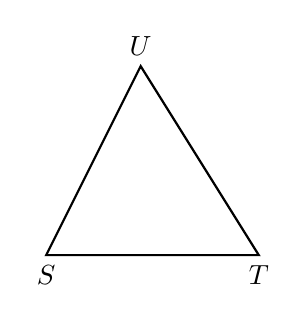
\begin{tikzpicture}[scale=0.3]
    \draw[thick] (0,0)node[below]{$S$}--
      (9,0) node[below]{$T$}--
      (4,8) node[above]{$U$}--cycle;
  \end{tikzpicture}
  \end{center}
  \end{frame}

\begin{frame}{An \emph{equilateral} triangle has all three sides congruent}
  Given equilateral $\triangle PQR$ with $PQ=2x-4$, $PR=10$. Find $x$.
  \begin{center}
  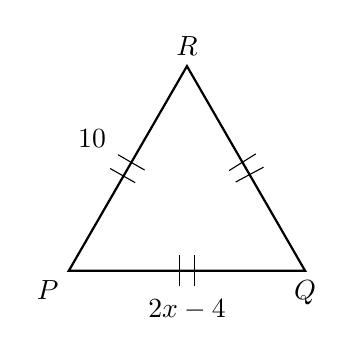
\begin{tikzpicture}[scale=1]
    \draw[thick] (0,0)node[below left]{$P$}--
      (3,0) node[below]{$Q$}--
      (60:3) node[above]{$R$}--cycle;
    \draw (1.4,-0.2)--(1.4,0.2);
    \draw (1.6,-0.2)--(1.6,0.2);
    \draw (53:1.4)--(68:1.4);
    \draw (53:1.6)--(67:1.6);
    \draw (28:2.4)--(28:2.8);
    \draw (32:2.4)--(32:2.8);
    \node at (80:1.7){10};
    \node at (1.5, -0.5){$2x-4$};
  \end{tikzpicture}
  \end{center}
  The \emph{perimeter} is the distance around the triangle. Find the perimeter of $\triangle PQR$. \vspace{1cm}
  \end{frame}

\begin{frame}{A \emph{quadrilateral} has four sides}
  Given two \emph{adjacent} equilateral $\triangle$s, $\triangle ABC$ and $\triangle ACD$. All sides measure 10 cm. 
  \begin{center}
  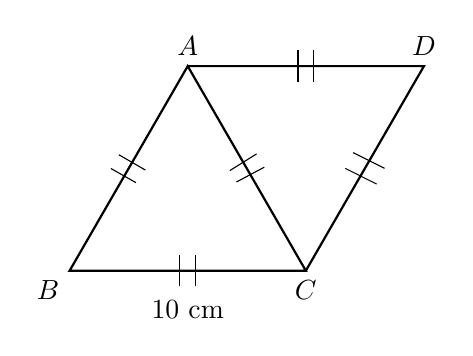
\begin{tikzpicture}[scale=1]
    \draw[thick] (0,0)node[below left]{$B$}--
      (3,0) node[below]{$C$}--
      (60:3) node[above]{$A$}--cycle;
    \draw (1.4,-0.2)--(1.4,0.2);
    \draw (1.6,-0.2)--(1.6,0.2);
    \draw (53:1.4)--(68:1.4);
    \draw (53:1.6)--(67:1.6);
    \draw (28:2.4)--(28:2.8);
    \draw (32:2.4)--(32:2.8);
    \draw[thick] (3,0)--
      (30:{3*1.732}) node[above]{$D$}--(60:3);
    \draw (2.9,2.4)--(2.9,2.8);
    \draw (3.1,2.4)--(3.1,2.8);
    \draw (3.5,1.3)--(3.9,1.1);
    \draw (3.6,1.5)--(4.0,1.3);
    \node at (1.5, -0.5){$10$ cm};
  \end{tikzpicture}
  \end{center} \bigskip
  Find the perimeter of the quadrilateral $ABCD$. \vspace{3cm}
  \end{frame}

\begin{frame}{Check your notes}
  \begin{description}
    \item[Equilateral] Triangle with all three sides congruent
    \item[Isosceles] Triangle having two sides of the same length
    \item[Scalene] Triangle without any sides of matching lengths
    \item[Quadrilateral] A four-sided figure (examples: square, rectangle, parallelogram, rhombus, kite)
    \item[Polygon] Objects with multiple sides (e.g. triangle, quadrilateral, pentagon, hexagon)
    \item[Perimeter] The total length around a figure (all sides added)
    \item[Adjacent] ``next to'', two things that are side by side
  \end{description}
\end{frame}

\begin{frame}{Spicy: Given the midpoint, find an end point}
  Points $A(1)$, $M(4)$, and $B$ lie on a numberline. $M$ bisects $\overline{AB}$. \par \medskip
  Find $B$.
  \begin{center}
    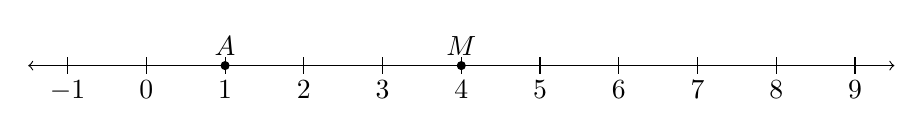
\begin{tikzpicture}
      \draw[<->] (-1.5,0)--(9.5,0);
      \foreach \x in {-1,...,9}
        \draw[shift={(\x,0)}] (0pt,-3pt)--(0pt,3pt) node[below=5pt]{$\x$};
      \draw[fill] (1,0) circle [radius=0.05] node[above]{$A$};
      \draw[fill] (4,0) circle [radius=0.05] node[above]{$M$};
    \end{tikzpicture}
  \end{center}\vspace{2cm}
  \end{frame}

\section{1.6 Roundtable review \hfill 16 September}
\begin{frame}{Learning Target: I can collaborate in review}
  {CCSS: HSG.CO.A.1 Know precise geometric definitions  \hfill \alert{1.6 Friday 16 September}}
  Do Now: Given the points $X$ and $Y$, draw $\overrightarrow{YX}$. \par \bigskip
  (careful! which direction does it go?) 
  \vspace{1cm}
  \begin{center}
    \begin{tikzpicture}
    \draw[fill] (1,2) circle [radius=0.05] node[below]{$X$};
    \draw[fill] (5,0) circle [radius=0.05] node[below]{$Y$};
  \end{tikzpicture}
  \end{center} \vspace{1cm}
  Lesson: Roundtable quiz review
\end{frame}

\begin{frame}{Groupwork review for \alert{quiz Monday}}
  {``Roundtable'' of four students, with four topics assigned}
  \begin{block}{Geometry skills to study / teach}
      \begin{enumerate}
    \item Conventions: terminology, notation, diagramming
    \item Modeling situations with algebra
    \item Perimeter and special shapes: 
    \begin{itemize}
      \item Scalene, isosceles, and equilateral $\triangle$s
      \item Squares, rectangles, parallelograms, trapezoids, rhombuses, kites \par 
      (quadrilateral side $\cong$s will be marked)
    \end{itemize}
    \item Solving algebraic equations for one variable
  \end{enumerate}
  \end{block}
  Problem sets are \alert{due Monday}, start of class: Inventory checklist on top, reverse chronological order, stapled. 
  \end{frame}

\begin{frame}{1. Identify each item.}
  {Example of Topic 1: Conventions: terminology, notation, diagramming}
  \begin{enumerate} 
    \item The point $A$
    \item The ray $\overrightarrow{BD}$
    \item The name of the plane
    \end{enumerate} \vspace{1cm}
    \begin{center}
      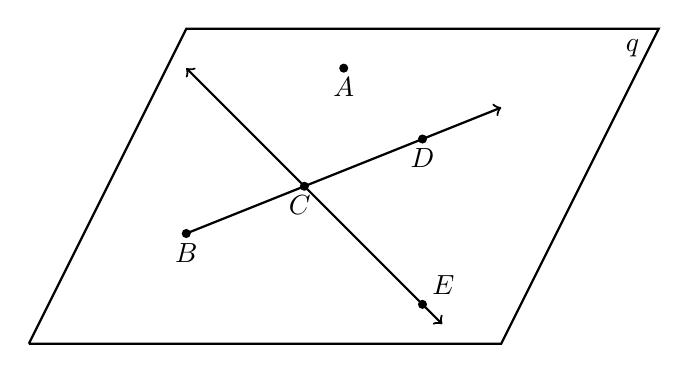
\begin{tikzpicture}
      \draw[thick](0,0)--(6,0)--(8,4) node[below left]{$q \ $} --(2,4)--(0,0);
      \draw[->, thick] (2, 1.4)--(6,3);
      \draw[fill] (4, 3.5) circle [radius=0.05] node[below]{$A$};
      \draw[fill] (2, 1.4) circle [radius=0.05] node[below]{$B$};
      \draw[fill] (3.5,2) circle [radius=0.05] node[below]{$C \ $};
      \draw[fill] (5,2.6) circle [radius=0.05] node[below]{$D$};
      \draw[<->, thick] (2,3.5)--(5.25,.25);
      \draw[fill] (5,0.5) circle [radius=0.05] node[above right]{$E \ $};
    \end{tikzpicture}
  \end{center}
  \end{frame}

\begin{frame}{2. Write down an equation to represent the situation}
  {Example of Topic 3: Modeling situations with algebra}
  Given $M$ is the midpoint of $\overline{AB}$, $AM=4x+2$, $AB=20$. \par \medskip
  \emph{First mark the diagram with hash marks and values.} \vspace{1cm}
    \begin{center}
      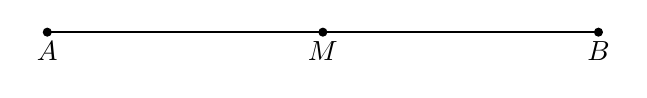
\begin{tikzpicture}
        \draw[fill] (0,0) circle [radius=0.05] node[below]{$A$};
        \draw[thick] (0,0)--(7,0);
        \draw[fill] (3.5,0) circle [radius=0.05] node[below]{$M$};
        \draw[fill] (7,0) circle [radius=0.05] node[below]{$B$};
      \end{tikzpicture}
    \end{center} \vspace{2cm}
  \emph{Sometimes you will not be asked to solve the equation.}
  \end{frame}
  
\begin{frame}{3. Find the perimeter of the rectangle $ABCD$}
  {Example of Topic 2: Perimeter and special triangles and quadrilaterals}
  Given $AB=6$ inches, $BC=4$ inches.
  \begin{center}
    \begin{tikzpicture}
    \draw[thick]
      (0,0)node[below left]{$A$}--
      (6,0)node[below right]{$B$}--
      (6,4)node[above right]{$C$}--
      (0,4)node[above left]{$D$}--cycle;
    \node at (3,-0.5){$6$ inches};
    \node at (6.6,2.3){$4$ in};
    \draw (2.9, -0.2)--(2.9,0.2);
    \draw (2.9, 3.8)--(2.9,4.2);
    \draw (-0.2, 1.9)--(0.2, 1.9);
    \draw (-0.2, 2.1)--(0.2, 2.1);
    \draw (-0.2, 1.9)--(0.2, 1.9);
    \draw (-0.2, 2.1)--(0.2, 2.1);
    \draw (5.8, 1.9)--(6.2, 1.9);
    \draw (5.8, 2.1)--(6.2, 2.1);
    \end{tikzpicture}
  \end{center}
  \end{frame}

\begin{frame}{4. Solve for $x$}
  {Example of Topic 4: Solving algebraic equations for one variable}
  Given $\overline{LMN}$, $LM=3x+1$, $MN=7$, $LN=17$.
    \begin{flushleft}
      \begin{tikzpicture}
      \draw[thick] (0,0)--(7,0);
      \draw[fill] (0,0) circle [radius=0.05] node[below]{$L$};
      \draw[fill] (4,0) circle [radius=0.05] node[below]{$M$};
      \draw[fill] (7,0) circle [radius=0.05] node[below]{$N$};
      \node at (1.7,0) [above]{$3x+1$};
      \node at (5.5,0) [above]{$7$};
      \draw[<->, dashed] (0,-1)--(7,-1);
      \node at (3.5,-1) [below]{$17$};
      \end{tikzpicture}
    \end{flushleft}
  \large \[ (3x+1)+7=17 \] \par \vspace{2cm}
  \emph{You must check the solution.}
  \end{frame}

\section{1.7 Unit conversion, Exit note quiz \hfill 19 September}
\begin{frame}{Learning Target: I can change units of length}
  {CCSS: HSG.CO.A.1 Know precise geometric definitions  \hfill \alert{1.7 Monday 19 September}}
  Do Now: Mike is six feet tall. How many inches is that? \par \medskip
  Conversion: 1 foot = 12 inches \par
  \vspace{3cm}
  \alert{Exit note quiz today}
  \end{frame}

\begin{frame}{Multiply by \emph{conversion factors} to change units}
  {reference: \href{https://en.wikipedia.org/wiki/Dimensional_analysis}{Wikipedia Dimension analysis}}
  Mike is six feet tall. How many inches is that? \par \medskip
  $$H = 6 \,\mathrm{feet} \times \displaystyle \frac{12 \,\mathrm{inches}}{1 \,\mathrm{foot}} = 72 \,\mathrm{inches}$$
  \begin{description}
    \item[Conversion factor] is a ratio of units equal to one, for example, 
  \end{description}
  $$\displaystyle \frac{12 \,\mathrm{inches}}{1 \,\mathrm{foot}} = 1$$
    \vspace{3cm}
  \end{frame}

\begin{frame}{Numerator vs denominator of conversion factors}
  An American football field is 100 yards long. How many feet is that?  \par \smallskip
  $$1 \,\mathrm{yard} = 3 \,\mathrm{feet}$$ \par \medskip
  \onslide<2> $$L = 100 \,\mathrm{yards} \times \displaystyle \frac{3 \,\mathrm{feet}}{1 \,\mathrm{yard}} = 300 \,\mathrm{feet}$$ \par \vspace{1cm}
  Each conversion factor ratio has two forms: \par \medskip
  $$\displaystyle  \frac{1 \,\mathrm{yards}}{3 \,\mathrm{feet}} = \frac{3 \,\mathrm{feet}}{1 \,\mathrm{yards}} = 1$$
  \end{frame}

\begin{frame}{Cancel units when choosing correct conversion factor}
  {reference: \href{https://www.nysedregents.org/geometryre/622/geom62022-exam.pdf}{NY State Regents Exam formula sheet}}
  Stephen's height is $H=69$ inches. Find his height in meters. \par \smallskip
   $$1 \,\mathrm{meter} = 39.37 \,\mathrm{inches}$$ \par \medskip
   \onslide<2> $$H = 69 \,\mathrm{inches} \times \displaystyle \frac{1 \,\mathrm{meter}}{39.37 \,\mathrm{inches}} = 1.7526\dots \,\mathrm{meter}$$ \par \vspace{1cm}
    Select the ratio with inches in the denominator: \par \medskip
      $$\displaystyle  \frac{39.37 \,\mathrm{inches}}{1 \,\mathrm{meter}} = \frac{1 \,\mathrm{meter}}{39.37 \,\mathrm{inches}} = 1$$
  \end{frame}


\end{document}